\section{Fysisk Lag}
Det fysiske lag er det nederste lag i systemet. Det står for at interagere med hardwaren og levere data til datalinklaget. 

\subsection{Mediet}
Transmissionsmediet, som anvendes til at sende data, er lyd i form af DTMF-toner. Der findes 16 forskellige DTMF-toner. Ud fra emperiske målinger er den mest stabile(se \ref{sec:hastighedstest}) sendetid fastlagt til at være 25 ms. per tone for at en tone bliver afkodet på modtagersiden. Dette giver en båndbredde begrænsning på 40 Hz.

\subsection{SFML}
Til at afsende og optage lyd bruges der et bibliotek kaldet "Simple and Fast Multimedie Library" forkortet SFML. Dette bibliotek er skrevet i C++ og indeholder funktioner til at interagere med hardwaren, uden at skulle rode med at initialisere og opsætte hardwaren. Biblioteket er opdelt i forskellige underbiblioteker alt efter, hvilken del af computerens hardware der skal interageres med. Og der kan derfor nøjes med kun at inkludere den funktionalitet, der er ønsket i projektet. Biblioteket er veldokumenteret på deres hjemmeside, hvor der også findes adskillige tutorials til, hvordan de forskellige funktioner bruges.

\subsection{Kodning}
For at kunne sende data over mediet, skal der vælges en linjekodning der fastsætter, hvor mange dataelementer som repræsenteres af et signalelement. Dataraten er det antal bits der kan sendes på et sekund og signalraten er det antal signalelementer der sendes på et sekund. Målet med linjekodningen er at øge dataraten og sænke signalraten. Da en øget datarate øger hastigheden af kommunikationen og en sænket signalrate sænker niveauet for båndbredde på mediet. Hvis en DTMF-tone anses for at være et signalelement så vil der med et signalelement kunne opnås $16^{1}$ mulige kombinationer af signalelementer. Hvis dataelementerne uddeles en til en på signalelementerne medfører dette at et dataelement indeholder $\sqrt{16}=4$ bits information. Dette giver at forholdet mellem dataelementer og signalelementer er $r=4$. Ud fra den båndbredde-begrænsning der er bestemt giver dette en bitrate på $N=40*4=160bps$. Dette er den hurtigste linjekodning der kan implementeres, og indeholder ingen ekstra signalelementer i forhold til dataelementer. Så der er ikke mulighed for at implementere fejltjek i forbindelse med linjekodningen. Ud fra tests blev der fundet ud af, at hardwaren og softwaren fint kan kende forskel på de 16 DTMF-toner. Så der vil fint kunne anvendes denne hurtige linjekodning til at få så meget data igennem på som muligt. Denne linjekodning er blevet valgt da den fungerer godt sammen med DTMF-tonerne. I tabel \ref{DTMFBitTabel} kan kortlægning af hvilke DTMF-toner der svarer til hvilke bit sekvenser ses.

\begin{table}[]
\centering
\caption{Bitmønster til DTMF}
\label{DTMFBitTabel}
\begin{tabular}{|c| c c c c|}
\hline
\multicolumn{1}{|l|}{DTMF Tone} & \multicolumn{4}{l|}{Bitmønster}                                                                   \\ \hline
0 								& 0						 & 0					  & 0
& 0						 \\ \hline
1 								& 0						 & 0					  & 0
& 1						 \\ \hline
2								& 0						 & 0					  & 1
& 0						 \\ \hline
3                               & 0                      & 0                      & 1                      & 1                      \\ \hline
4                               & 0                      & 1                      & 0                      & 0                      \\ \hline
5                               & 0                      & 1                      & 0                      & 1                      \\ \hline
6                               & 0                      & 1                      & 1                      & 0                      \\ \hline
7                               & 0                      & 1                      & 1                      & 1                      \\ \hline
8                               & 1                      & 0                      & 0                      & 0                      \\ \hline
9                               & 1                      & 0                      & 0                      & 1                      \\ \hline
A                               & 1                      & 0                      & 1                      & 0                      \\ \hline
B                               & 1                      & 0                      & 1                      & 1                      \\ \hline
C                               & 1                      & 1                      & 0                      & 0                      \\ \hline
D                               & 1                      & 1                      & 0                      & 1                      \\ \hline
*                               & 1                      & 1                      & 1                      & 0                      \\ \hline
\#                              & 1                      & 1                      & 1                      & 1                      \\ \hline
\end{tabular}
\end{table}

\subsection{Fejl-kontrol}
Der er ikke implementeret nogen form for fejl-kontrol i det fysiske lag. Linjekodningen koder dataelementer en til en med signalelementer. Så hvis der sker en fejl vil denne altid ende ud i at der modtages et forkert bitmønster. Disse fejldata sendes videre til datalinklaget, som skal finde fejlen.

\subsection{Flow-kontrol}
Det fysiske lag implementerer ikke nogen form for flow-kontrol. Så snart data kommer ned til laget bliver det sendt afsted uden at tjekke om mediet er optaget. På modtagersiden bliver der konstant lyttet efter data og i det øjeblik data modtages, placeres det i et buffer som datalinklaget kan hente fra. Dette sker uanset om datalinklaget er travlt beskæftiget eller ej og bufferen er kun begrænset af den fysiske hukommelse i den maskine der kører softwaren.

\subsection{Afsender}
Afsenderen modtager en vektor af booleans fra datalinklaget. Denne vektor omdannes til DTMF-toner og ud fra disse DTMF-toner genererer generator klassen den lydfil, som bliver afspillet over højtalerne.

\subsubsection{Transmitter}
Transmitterklassen er den primære klasse i det fysiske lag. Klassen står for at konvertere binær data i form af en \textit{vektor$<$bool$>$} om til en \textit{vektor$<$DTMF::Tone$>$} og sende denne nye vektor videre til \textit{generator} klassen, som behandler data og returnerer en lyd indeholdende de ønskede DTMF-toner. Denne lyd kan så afspilles via et  \textit{sf::Sound} objekt.

\subsubsection{Generator}
Generator klassen er den klasse der står for at generere den lyd der skal afspilles. Klassen har en central funktion der genererer lyden kaldet \textit{generate}. Funktionen tager en vektor af \textit{DTMF::Tone} og returnerer en pointer til et \textit{sf::SoundBuffer} objekt. Dette objekt kommer fra SFML og kan bruges til at definere en lyd ud fra et array af heltal og en samplerate. Selve \textit{generate} funktionen tager DTMF-tonerne en af gangen og slår op i en tabel, hvilke frekvenser den pågældende tone indeholder. Ud fra dette kan den så generere to sinus der overlejres med hinanden og multipliceres med en volumen. Hvis volumen er sat til en fast værdi, så vil der opstå et brat skift imellem DTMF-tonerne grundet at en tone starter i fase 0 og dette bratte skift resulterer i at højtaleren laver en pop-lyd. Til at undgå dette er der implementeret forskellige funktioner til at modulerer den volumen der ganges på sådan så overgangen mellem DTMF-tonerne kan justeres til at være blød. Der kan læses om de forskellige overgange i afsnit \ref{sec:ToneTransition}




\subsection{Receiver}
Receiveren er en samling af flere klasser, som tilsammen sørger for at optage lyd og afkode alle DTMF-toner der bliver modtaget. Tonerne bliver konverteret til en vektor af bools, som datalinklaget kan pulle fra.

\subsubsection{Goertzel}

For at afgøre om bestemte frekvenser er til stede i et signal anvendes Goertzel-algoritmen. Den kan returnere en magnitude, hvis størrelse afhænger af hvor meget signalet man giver, korrelerer med bestemte frekvenser. På den måde kan man se på om den returnerede magnitude er over en bestem grænseværdi, for at afgøre om den ønskede frekvens er til stede i signalet. 
For at konvertere til diskrete frekvenser bruges formel \eqref{eq:targetBin} og \eqref{eq:omega} - k beskriver hvilken bin targetfrekvensen ligger i, og $\omega$ er den normaliserede frekvens. k skal afrundes til et heltal.

\noindent\begin{minipage}{.5\linewidth}
\begin{equation} \label{eq:targetBin}
 k=N*\dfrac{targetFrekvens}{Samplerate}
\end{equation}
\end{minipage}%
\begin{minipage}{.5\linewidth}
\begin{equation}
\label{eq:omega}  
\omega = \dfrac{2*\pi}{N}*k
\end{equation}
\end{minipage}


Fordelen ved at anvende Goertzel-algoritmen frem for en DFT/FFT er, at man kan nøjes med kun at kigge på nogle få frekvens-bins ad gangen, og så derfra finde DFT-koefficienten for den bin alene. Den udregning er langt nemmere at foretage, så længe man kun er interesseret i relativt få frekvenser. Selve algoritmen kommer fra et 2. ordens IIR-båndpas-filter, med en pol og dens konjugerede placeret på enhedscirklen i de bins, hvor man leder efter frekvenser (se ligning \eqref{eq:transferfunction}) En anden ting der taler for Goertzel-algoritmen i vores tilfælde, er at de tungeste udregninger kan foretages på forhånd, og gemmes som konstanter i en tabel, man så kan slå op i. I goertzel-klassen foretages det tunge arbejde i en initialiseringsfunktion \textit{init()}, der regner alle konstanter til hver frekvens og gemmer dem i et map, man så kan slå op i med den ønskede frekvens. For at lave udregningerne, skal man bare kende samplingfrekvensen og antallet af samples man regner med at bruge i selve algoritmen - det vil i vores tilfælde være sampleWindow. Der udregnes også en skaleringsfaktor, der skal ganges på DFT-koefficienten's magnitude for at finde det en-sidede amplitudespektrum. Amplitudespektret vil være den værdi, man kigger på for at afgøre om en frekvens er til stede i et signal. 
Overføringsfunktionen til Goertzel-filteret:



\begin{equation}\label{eq:transferfunction}
H(z) = \frac{1}{1-2Cos(\omega)z^{-1}+z^{-2}}
\end{equation}


I goertzel-klassen foretages det tunge arbejde i en initialiseringsfunktion \textit{init()}, der regner alle konstanter til hver frekvens og gemmer dem i et map, man så kan slå op i med den ønskede frekvens. \\
Når selve algoritmen bliver brugt, køres alle samples igennem filteret og derefter regnes magnitude ud, fra den reelle og den imaginære del af DFT-koefficienten.





\subsubsection{Recorder}

Recorderen kommer fra SFML-biblioteket. Det er muligt at designe sin egen recorder-klasse, ved at arve fra en af de indbyggede klasser og så overloade tre funktioner der returnerer bools. Funktionerne bruges til at fortælle superklasserne om de kan fortsætte med at udføre bestemte handlinger, man sætter igang med andre funktioner. Hvis de returnerer false stoppes handlingen og omvendt hvis de returnerer true.

\begin{itemize}

\item \textbf{onStart():} Bliver kørt når man beder om at starte en optagelse. Her kan man indsætte forskellige tests der afgør om det er smart at fortsætte med at starte optagelsen. Det kunne eksempelvis testes, om der overhovedet kan skabes kontakt til en mikrofon.

\item \textbf{onProcessSamples():} Funktionen får givet en pointer til samples og antallet af dem som parametre. Det er så muligt at flytte dem til sin egen buffer til videre behandling. Den bliver kørt med jævne mellemrum, når en optagelse er startet, og mellemrummet kan defineres med funktionen setProcessingInterval(). 

\item \textbf{onStop():} Bliver kørt når man beder om at stoppe en optagelse.

\end{itemize}

Der er sådan set en fungerende optagerklasse inkluderet i SFML-biblioteket fra starten af, men den er lidt mindre fleksibel, og nærmere tiltænkt brug som en slags plug-and-play optager. Det er ikke muligt løbende at trække samples ud af bufferen, hvis man er interesseret i at processere dem i real-time. Derfor er en custom recorder at foretrække i vores tilfælde. \\
Recorderen kører i sin egen tråd, parallelt med alt andet, så derfor skal man huske at låse delte resourcer med en mutex, for at forhindre data race situationer - det er nødvendigt når der læses fra eller skrives til bufferen. SFML har også sin egen mutex-klasse som bruges flere steder.

\subsubsection{Analyzer}

Analyzer-klassen fungerer som bindeled mellem recorderen og goertzel-klassen. Det er den der styrer behandlingen af de samples der kommer ind. Dens primære opgave er at søge sin buffer igennem for frekvenser, der indgår i DTMF-toner. Hvis den finder nogen, oversættes de til karakterer, der kan sendes videre i systemet. Analyzeren har sin egen buffer, som den kan arbejde på i fred. Når denne buffer er tømt, kan der hentes nye samples ind fra recorderens buffer. \\

Detektionen af DTMF-toner udføres af to funktioner - \textit{syncToFirstDTMF()} og \textit{findNextDTMF()}. De er designet ud fra den antagelse, at når der kommer beskeder ind, vil de altid komme i en strøm af toner adskilt af et lille mellemrum uden lyd. Så hvis man kan finde den første DTMF-tone i denne strøm, så kan man blive ved med at kigge på et antal samples frem i tiden, der svarer til længden af hver tone. Det kan nemt udregnes fra samplefrekvensen \eqref{eq:sampleWindow}. \\

\begin{equation}
sampleWindow=sampleRate[samples/s]*toneLaengde[s]
\label{eq:sampleWindow}
\end{equation}

\begin{figure}[h!]
\centering
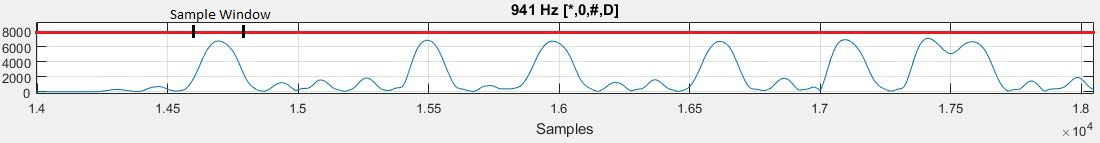
\includegraphics[scale=0.5]{Billeder/Samplewindow.PNG}
\caption{Her ses samplewindow, når det er stillet optimalt på den første tone. Magnitudes ved 941 Hz er vist op ad y-aksen}
\label{fig:Samplewindow}
\end{figure}

Når \textit{syncToFirstDTMF} leder bufferen igennem, er dens vigtigste opgave at stille sampleWindow mere eller mindre lige oveni den første DTMF-tone den finder, så magnitude på den næste gang samples er på sit højeste. På den måde kan \textit{findNextDTMF} blive ved med at kigge på et sampleWindow, finde tonen og så slette alle de analyserede samples fra bufferen uden at bekymre sig om, hvorvidt man har slettet for meget af en anden tone. Inden den første tone er fundet, slettes der kun 1/4 af sampleWindow ad gangen, så man ikke risikerer at slette nogle vigtige samples. Første gang man støder på en tone, søges et område á to sample vinduer i nærheden igennem, for at finde den position, hvor magnituden for den fundne karakter er størst. Den viden kan så bruges til at bestemme nogenlunde præcist, hvor mange samples der skal slettes, for at det næste vindue står lige oveni en tone. På transmittersiden, er der sørget for at volumen er højest midt i en tone ved at gange et slags vindue på - på den måde kan man godt antage, at magnitude fra goertzel-algoritmen er højest cirka midt i tonen.

\paragraph{Synkronisering af grænseværdier}\hfill \break

Magnituden for de anvendte frekvenser varierer en del afhængigt af modulationen på afsendersiden, afstanden og vinklen imellem mikrofon og højtaler. Derudover påvirkes magnitude i forskellig grad for hver frekvens (se \ref{sec:afstand}). Det vil derfor være meget svært at programmere en fast grænseværdi på forhånd, medmindre det er til meget bestemte fysiske forhold. En bedre løsning er at synkronisere grænseværdien løbende mens programmet kører, så programmet bliver mere stabilt og kan anvendes i flere situationer.

\begin{figure}[h!]
\centering
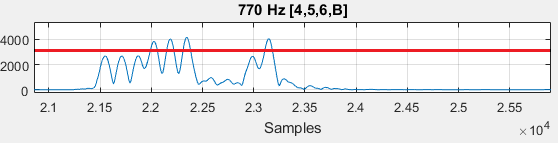
\includegraphics[scale=0.7]{Billeder/Threshold.PNG}
\caption{Den røde linje viser grænseværdien. Hvis magnitude for en række samples er større end grænseværdien, kan det antages at en frekvens på 770 Hz er til stede i de samples}
\label{fig:threshold}
\end{figure}

Idet grænseværdien kan variere for alle frekvenser, vil det være nødvendigt at have en grænseværdi til hver frekvens. I praksis er det gjort med et map, hvor hver grænseværdi er gemt med frekvensen som nøgle. Et map er en container fra standardbiblioteket, hvor man kan referere en datatype med en nøgle som man selv kan definere. Nøglen kan være stort set hvilken som helst datatype. PhysicalReceive-klassen holder styr på, om alle frekvenser er opdateret, i et map med bools med frekvenserne som nøgle. Når disse bools er \textit{false} finder analyzeren den største magnitude til frekvenserne, og sætter den nye grænseværdi til 75 \% af den værdi (På figur \ref{fig:threshold} er grænseværdien ca 75 \% af max, og det er lige på kanten af hvad der er optimalt, da det kun er de største peaks, der skal regnes som steder, hvor 770 Hz er til stede). Mappet med bools er designet så det løbende bliver opdateret, i takt med at de specifikke frekvenser bliver modtaget. 

\subsubsection{Physical Receive}

PhysicalReceive-klassen har til opgave at styre hvordan hele analyseringsprocessen forløber, og så i sidste ende sende en vektor med bools op til datalink-laget til videre behandling. Da denne klasse er forbindelsen til de øvre lag, er der her lavet funktioner til at starte og stoppe recorderen. Funktionen \textit{continuousAnalysis()} kan køre i sin egen tråd, og sørger for at bufferen i Analyzer-klassen løbende bliver kigget igennem for DTMF-toner. Til styringen af analyzeren, er der to vigtige ting at holde øje med.

\begin{itemize}

\item \textbf{Hvornår bliver strømmen af toner brudt.} Lige så snart der ikke kan findes flere toner sættes en bool, \textit{charStringBroken}, der fortæller Analyzeren at den er nødt til at synkronisere igen. Så længe denne bool ikke er sat, fortsætter Analyzeren med at kigge på samples en gang, returnere den fundne tone og så slette dem igen. 
\item \textbf{Hvornår er bufferen ved at være tømt.} Når bufferen når under en størrelse af 4 samplewindows, må der ikke foretages mere, før der er fyldt nye samples i fra recorderen. På den måde bryder man ikke den synkronisering, der er lavet en gang, og det forhindrer også funktionen i at forsøge at indeksere uden for bufferen.
\end{itemize}

De to første toner i en hvilken som helst sammenhængende strøm bliver ignoreret, da det altid vil være en preamble. Preamblen er lavet for at gøre synkroniseringen nemmere. Vi valgte DTMF-tonerne 'A' og '6' da de ikke har nogen overlappende frekvenser - tests vi lavede viste, at magnitude for en frekvens, der fandtes i to toner lige ved siden af hinanden, ikke faldt ret meget imellem tonerne. Det havde den effekt at sampleWindow kunne stå forkert selv efter synkroniseringen. Problemet er sidenhen blevet gjort mindre af at gange et Hann-Window på samples i goertzel-algoritmen (se \ref{sec:Windowfunction}), men preamblen bliver stadig brugt. 


Alle toner der ikke er en del af preamblen, bliver konverteret til bools og placeret i en vektor, \textit{boolsReceived}, der fungerer som bindeledet imellem det fysiske, og datalinklaget. I kraft af at de to lag kører i hver sin tråd er det nødvendigt at låse \textit{boolsReceived} med en mutex, for at forhindre data race situationer. Det gøres i praksis ved at låse funktionerne \textit{addNibble()} og \textit{extractBools()}, der henholdsvis skriver til og læser fra vektoren. Datalinklaget trækker selv bools fra det fysiske lag, når det er klart til det.\\